\chapter{Beschreibung des Systems}\label{ch:Systembeschreibung}
Diese Arbeit beschäftigt sich mit der Modellierung und Simulation eines Doppelpendels und eines Dreifachpendels. 

Das Doppelpendel besteht aus zwei Pendeln, die an einem gemeinsamen Punkt aufgehängt sind. Die Abbildung \ref{fig:Doppelpendel} zeigt das System mit den relevanten Größen. Die Längen $l_1$ und $l_2$ der Pendelarme sowie die Massen $m_1$ und $m_2$ der Pendel sind dargestellt. Die Abbildung zeigt auch die Abstände $s_1$ und $s_2$, die die Abstände der Massen von den Aufhängepunkten beschreiben. Die Gravitationskonstante $g$ und die Trägheitsmomente $J_1$ und $J_2$ der Pendel sind ebenfalls angegeben. Außerdem sind die Winkel $\varphi_1$ und $\varphi_2$ eingezeichnet, die die Lage der Pendel relativ zur Vertikalen beschreiben. Die Abbildung zeigt auch die Positionen $x_1$, $y_1$, $x_2$ und $y_2$, die die Endpunkte der Pendel darstellen. 

Das Dreifachpendel besteht aus drei Pendeln, die ebenfalls an einem gemeinsamen Punkt aufgehängt sind. Die Abbildung \ref{fig:Dreifachpendel} zeigt das System mit den relevanten Größen. Die Längen $l_1$, $l_2$ und $l_3$ der Pendelarme sowie die Massen $m_1$, $m_2$ und $m_3$ der Pendel sind dargestellt. Die Abbildung zeigt auch die Abstände $s_1$, $s_2$ und $s_3$, die die Abstände der Massen von den Aufhängepunkten beschreiben. Die Gravitationskonstante $g$ und die Trägheitsmomente $J_1$, $J_2$ und $J_3$ der Pendel sind ebenfalls angegeben. Außerdem sind die Winkel $\varphi_1$, $\varphi_2$ und $\varphi_3$ eingezeichnet, die die Lage der Pendel relativ zur Vertikalen beschreiben. Die Abbildung zeigt auch die Positionen $x_1$, $y_1$, $x_2$, $y_2$, $x_3$ und $y_3$, die die Endpunkte der Pendel darstellen.

\begin{figure}[H]
  \centering
  \begin{subfigure}{0.47\textwidth}
    \centering
    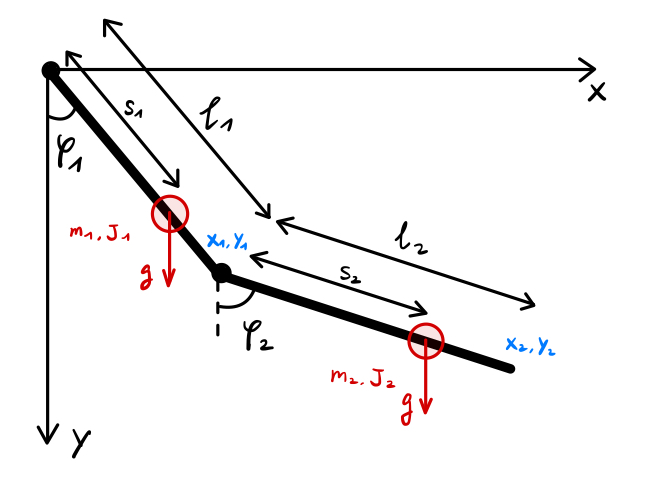
\includegraphics[width=\textwidth]{figures/Doppelpendel.png}
    \caption{Doppelpendel}
    \label{fig:Doppelpendel}
  \end{subfigure}
  \hfill 
  \begin{subfigure}{0.51\textwidth}
    \centering
    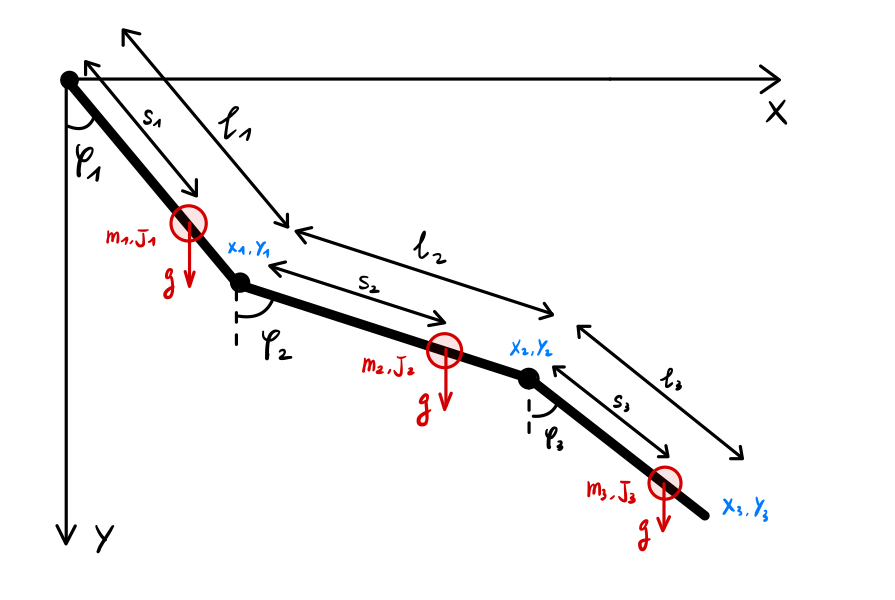
\includegraphics[width=\textwidth]{figures/Dreifachpendel.png}
    \caption{Dreifachpendel}
    \label{fig:Dreifachpendel}
  \end{subfigure}
  \caption{Doppelpendel und Dreifachpendel}
  \label{fig:Doppelpendel_Dreifachpendel}
\end{figure}





